%!TEX root = ../ShajiS_RnDReport.tex
\documentclass[../ShajiS_RnDReport.tex]{subfiles}

\begin{document}
\section{Evaluation}
\label{sec:evaluation}
% If your work involved experiments, describe the experimental setup and the results in this section.

The \glspl{vlm} are evaluated on the robotic vision task of image classification. First, the models are evaluated on the CIFAR-10 dataset for the task of generating pseudolabels under various prompting strategies. Then, the feasibility of training lightweight downstream models from the generated pseudolabels is assessed to determine if `knowledge' from larger \glspl{vlm} can be utilized for training such models. Finally, the performance of these lightweight models is analyzed in comparison to their counterparts that were trained on fully labeled, ground-truth datasets. This evaluation on the CIFAR-10 dataset is intended to be able to show how models can be transferred when they likely have knowledge of the task from pre-training. It aims to evaluate the effectiveness of few-shot learning in adapting to new tasks when the model already possesses knowledge of the concepts required for the task.

The performances of the \glspl{vlm} are then evaluated on a more specific dataset, namely the Seven-Point Checklist Dermatology Dataset (Derm7Pt)~\cite{Kawahara2019}. This dataset represents a task on which the \gls{vlm} would likely not have enough knowledge on from pre-training due to its specialized nature, and aims to evaluate the effectiveness various prompting strategies when the model likely does not possess knowledge of the concepts required for the task.

\subsection{CIFAR-10}
\label{subsec:evaluation:cifar10}
Four \glspl{vlm} were evaluated on CIFAR-10: Pixtral 12B, InternVL2, MiniCPM v2.6, and Phi-3.5 Vision Instruct. Each model was subjected to a series of experiments designed to assess their performance under different prompting strategies.

The analysis primarily encompassed zero-shot and few-shot experiments. An overview of experiment types is given in \autoref{tab:cifar_experiment_types}.

\begin{table}[ht]
    \centering
    \begin{tabular}{p{0.2\linewidth}p{0.6\linewidth}}
        \hline
        \textbf{Experiment Type} & \textbf{Description} \\
        \hline
        0-shot & Basic prompting with randomized class lists, no examples provided \\
        0.5-shot & 0-shot prompting enhanced with additional task-specific information \\
        Reasoning & 0-shot prompting with step-by-step reasoning requirements \\
        Few-shot & 1-16 examples provided without additional prompting \\
        Few-zero-shot & Few-shot examples combined with 0-shot prompting \\
        Few-five-shot & Few-shot examples combined with 0.5-shot prompting \\
        \hline
    \end{tabular}
    \caption{Overview of Experiment Types for the CIFAR-10 Experiment. Note that we refer to 0-shot and 0.5-shot experiments together as zero-shot experiments.}
    \label{tab:cifar_experiment_types}
\end{table}

\subsubsection{Evaluation Metrics}
The performance metric for the \glspl{vlm} on the CIFAR-10 dataset is primarily the basic accuracy. Basic accuracy is calculated as the simple percentage of correct predictions across all samples in the dataset. This metric gives a straightforward indication of how well the model is performing overall. However, it does not account for instances where the model generates invalid predictions -- those that cannot be matched to any class names in the CIFAR-10 class list and hence cannot be used for training a downstream model. In effect, this means that the effective accuracy of the pseudolabels seen by a downstream model during training can be different from this basic accuracy. A detailed formulation of the metrics can be found in Appendix \ref{sec:appendix:metrics:cifar10}. In the case of the downstream models, the metrics are computed without invalid predictions, as the downstream models, being trained on one-hot encoded labels for the class list, do not make invalid predictions.

\subsubsection{0-shot and 0.5-shot Performance}
The evaluation of 0-shot performance revealed a generally consistent level of effectiveness across various prompting strategies, as shown in \autoref{tab:cifar_zero_shot_performance}. However, it was observed that the introduction of reasoning requirements negatively impacted performance, resulting in a decrease of approximately 10-15\%. This can be attributed to the fact that the models were prompted to output the final answer in a certain format. While the answer would be parsed using several formats, some models omitted the generation of the final answer in one of the correct formats or at all, which means their answer would be classified as invalid and hence incorrect. Interestingly, downstream models that were trained using the generated zero-shot pseudolabels outperformed the \glspl{vlm} themselves. Notably, the best-performing downstream model, trained from pseudolabels generated by the MiniCPM model, achieved results that were only 5\% lower than the established baseline, as shown in \autoref{fig:cifar_downstream_model_accuracy_delta_few_zero_shot_over_few_shot}. The addition of task specific information in the 0-shot prompt (which we designate 0.5-shot) produces a minor improvement in performance for nearly no additional resource usage.

\input{tables/cifar_zero_shot_performance}

The analysis of memory usage indicated that all models maintained a constant memory footprint throughout the zero-shot experiments. On the other hand, the time requirements exhibited a notable increase when reasoning was incorporated into the prompting process, with time taken escalating by a factor of 10-35\% compared to scenarios where reasoning was not employed.

\subsubsection{Few-shot Performance}
Analysis of few-shot performance revealed a nuanced pattern of model improvement as the number of examples increased. Most models demonstrated an improving performance trend up to 8 shots, though typically not surpassing their best zero-shot performance levels. The pure few-shot experiment with 1-shot examples was particularly challenging, with a significant proportion of the incorrect predictions being invalid -- ranging from one-third to one-half of the dataset, depending on the \gls{vlm}. These invalid predictions stemmed from the \glspl{vlm} generating predictions outside the class list (due to the absence of a prompt or class list informing the model of it) that, while potentially reasonable classification of the images, did not match the required classification scheme.

The scaling behavior varied markedly across models. Pixtral 12B exhibited consistent performance gains up to 8 shots, while InternVL2 showed more modest but sustained improvements continuing up to 16 shots. Conversely, MiniCPM and Phi-3.5 reached their performance peaks earlier -- at 6 and 4 shots respectively -- after which their performance began to decline. The detailed performance metrics for these few-shot experiments are presented in \autoref{tab:cifar_few_zero_shot_performance}.

\input{tables/cifar_few_zero_shot_performance}

\paragraph*{Prompting Strategy Impact}
The analysis of different prompting strategies reveals that the addition of prompts in few-zero-shot experiments led to significant improvements in performance for low-shot scenarios with 1-4 examples, although these improvements did not generally surpass zero-shot performance levels. As the number of shots increased, the benefits provided by additional prompting diminished. Combining few-shot examples with either 0-shot or 0.5-shot prompting (in the form of few-zero- or few-five-shot experiments) consistently produces better performance compared to pure few-shot approaches. Given that the performance difference between few-five-shot and few-zero-shot configurations was minimal and sometimes negligible, a detailed analysis comparing these scenarios is omitted. This improvement in performance with added prompts can be seen in \autoref{fig:cifar_accuracy_delta_few_zero_shot_over_few_shot}, while \autoref{fig:cifar_downstream_model_accuracy_delta_few_zero_shot_over_few_shot} demonstrates the corresponding impact on downstream model performance. Looking at the bigger picture, \autoref{fig:cifar_experiment_best_results_scaled_by_model_parameter_count} provides a comprehensive comparison of model performances scaled by their respective parameter counts, which interestingly reveals that model size does not necessarily correlate with performance.

\begin{figure*}[ht]
    \centering
    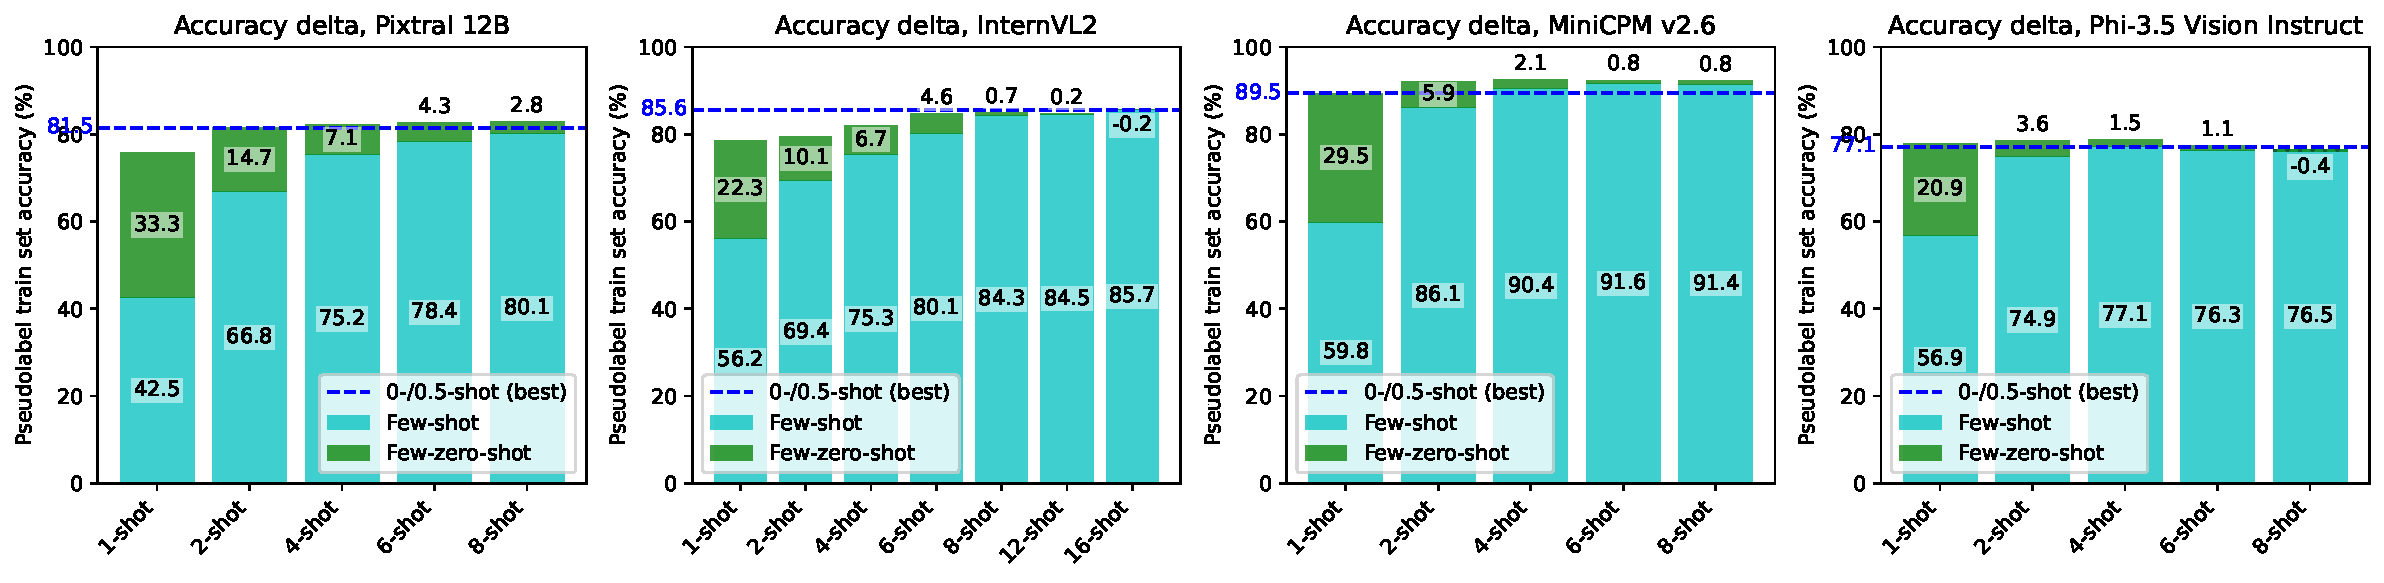
\includegraphics[width=\linewidth]{figures/cifar_accuracy_delta_few_zero_shot_over_few_shot.pdf}
    \caption{Visualization of delta of accuracies of few-zero-shot experiments over few-shot experiments -- adding prompts significantly improves performance in low-shot scenarios. Note that delta values can be negative, indicating that few-shot experiment results were better than few-zero-shot experiment results.}
    \label{fig:cifar_accuracy_delta_few_zero_shot_over_few_shot}
\end{figure*}

\begin{figure*}[ht]
    \centering
    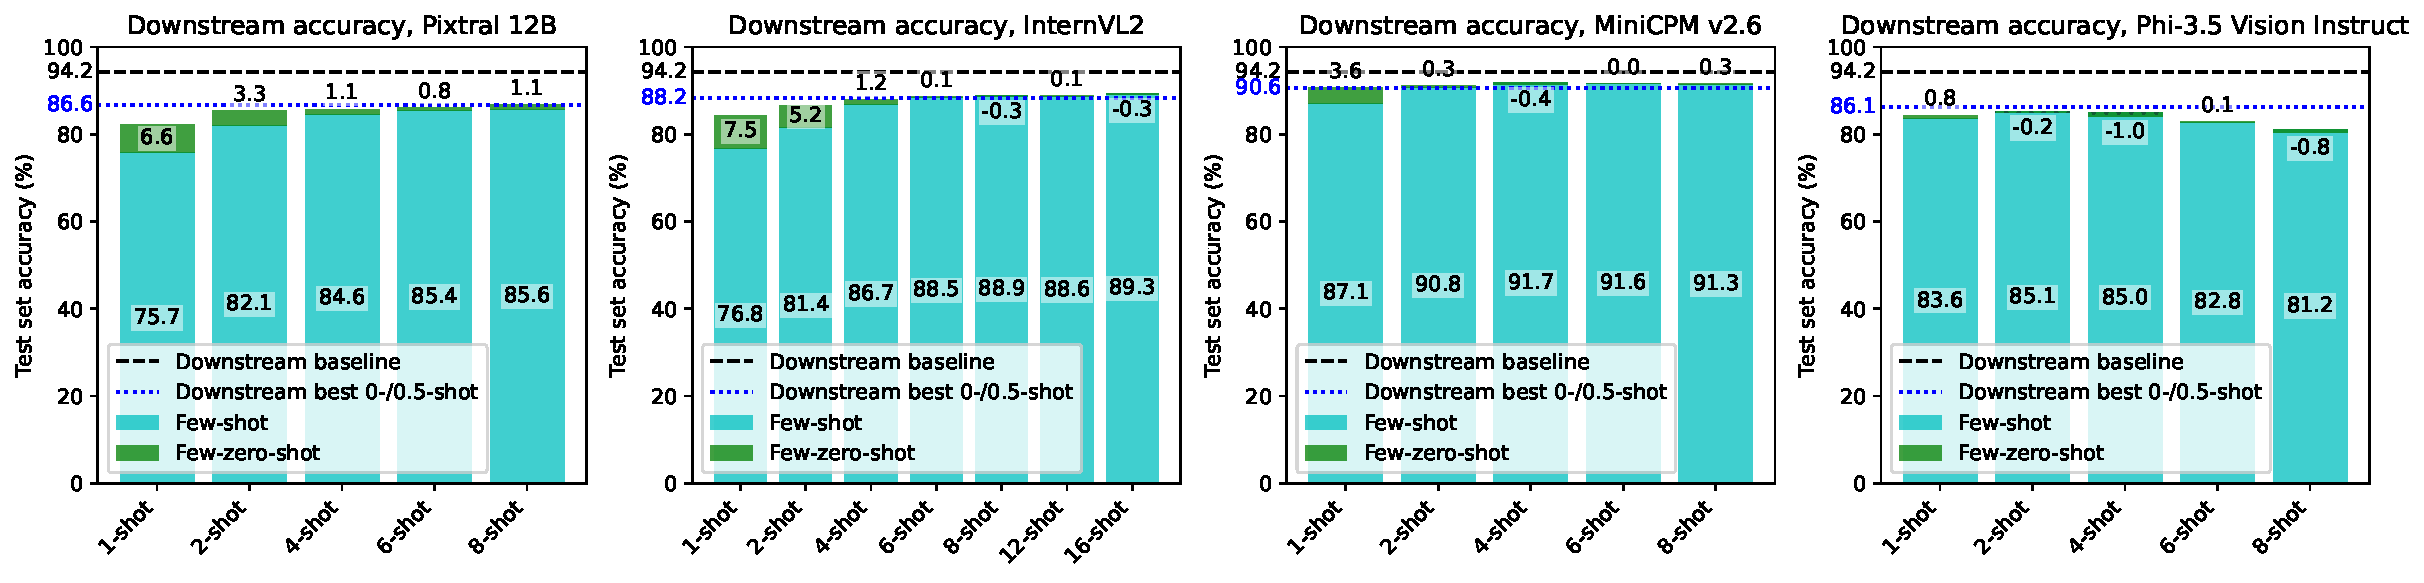
\includegraphics[width=\linewidth]{figures/cifar_downstream_model_accuracy_delta_few_zero_shot_over_few_shot.pdf}
    \caption{Visualization of delta of accuracies of downstream models on few-zero-shot experiments over few-shot experiments -- downstream models trained from few-zero-shot pseudolabels generally perform better than those trained from few-shot pseudolabels. However, the differences in performance of the downstream models are not as significant as that observed for the \glspl{vlm} themselves. Note that delta values can be negative, indicating that few-shot experiment results were better than few-zero-shot experiment results.}
    \label{fig:cifar_downstream_model_accuracy_delta_few_zero_shot_over_few_shot}
\end{figure*}

\begin{figure}[ht]
    \centering
    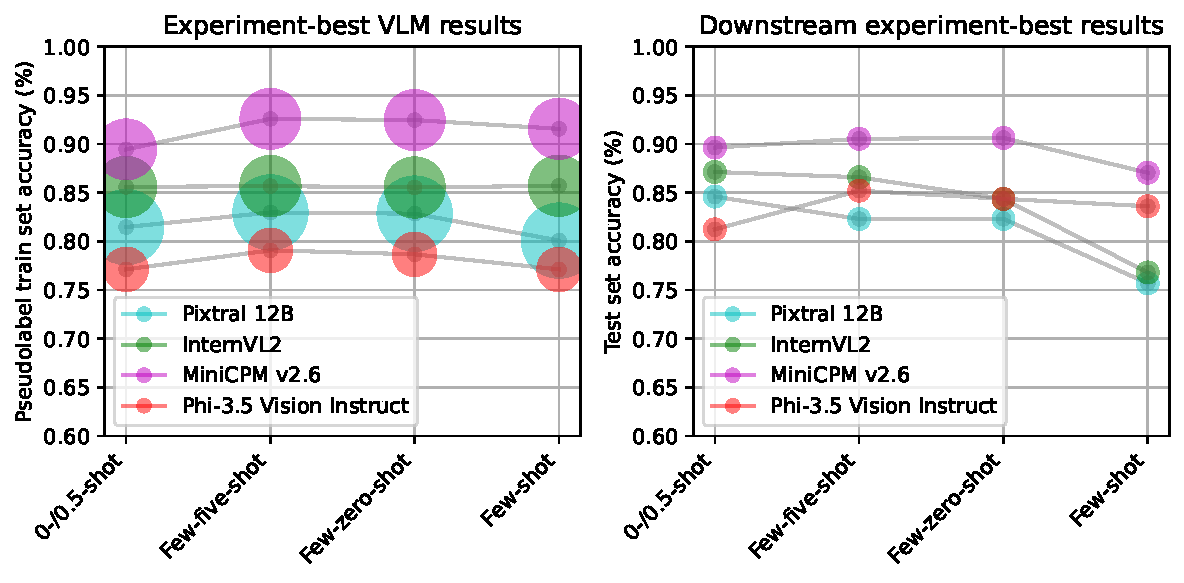
\includegraphics[width=\linewidth]{figures/cifar_experiment_best_results_scaled_by_model_parameter_count.pdf}
    \caption{Visualization of the best results for each experiment, which, in case of the \gls{vlm} experiments, are scaled by the model parameter count of the \gls{vlm}. Note that the parameter count is not directly indicative of the performance of the model, and the relative performances of the \glspl{vlm} do not necessarily correlate with the relative performances of the downstream models.}
    \label{fig:cifar_experiment_best_results_scaled_by_model_parameter_count}
\end{figure}

\subsubsection{Resource Requirements}
The analysis of computational resource requirements revealed distinct patterns in both memory and time usage across different models, as illustrated in \autoref{fig:cifar_few_shot_memory_usage_relative_to_zero_shot}. Notably, memory usage varied significantly among the models: Pixtral 12B exhibited a super-linear increase with additional shots, while InternVL2 and Phi-3.5 demonstrated linear scaling patterns. In contrast, MiniCPM maintained nearly constant memory usage, which may be attributed to its use of a perceiver-resampler architecture for image token processing. Note that the memory scaling expected from a pure Transformer architecture is quadratic~\cite{Vaswani2017}. The observed scaling patterns were even more pronounced in terms of processing time, where all models exhibited a super-linear increase as the number of shots increased. The impact was substantial and followed a clear progression: experiments with 2 shots took approximately 10 times longer than zero-shot scenarios, while 4 shots required about 20 times more processing time. Furthermore, 8-shot experiments demanded between 30 to 50 times more processing time compared to their zero-shot counterparts.

\begin{figure*}[ht]
    \centering
    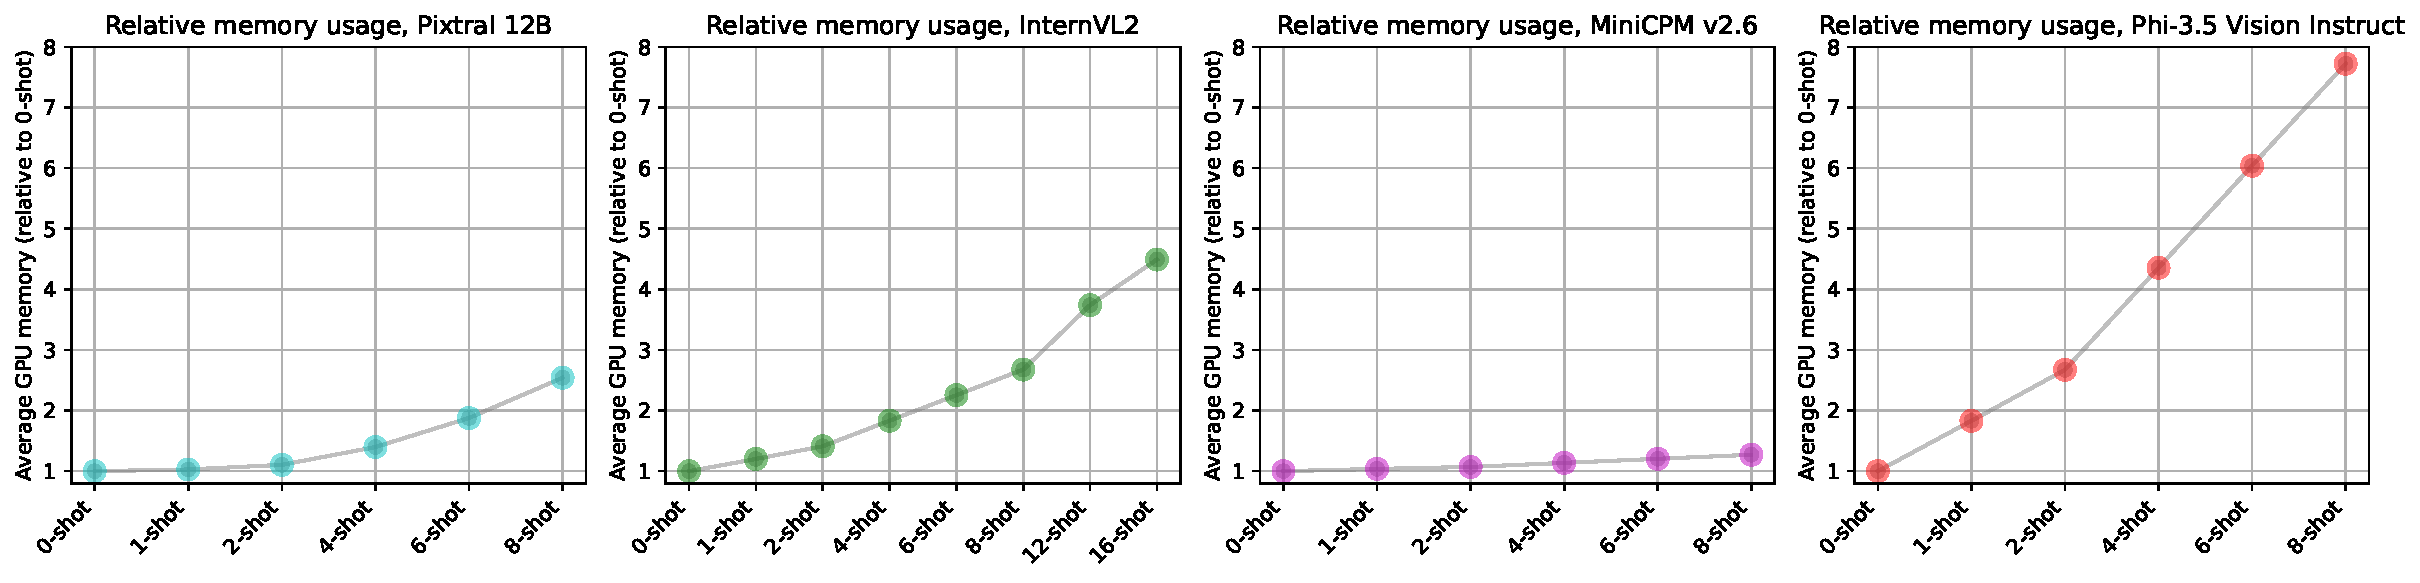
\includegraphics[width=\linewidth]{figures/cifar_few_shot_memory_usage_relative_to_zero_shot.pdf}
    \caption{Memory usage of \glspl{vlm} in few-shot experiments relative to zero-shot experiments -- most models investigated here show a super-linear increase in memory usage with the number of shots. The average time required for processing each example from the dataset also shows a comparable trend, albeit with a strictly higher growth with the number of shots.}
    \label{fig:cifar_few_shot_memory_usage_relative_to_zero_shot}
\end{figure*}

\subsubsection{Downstream Model Analysis}
The performance of the downstream models is analyzed to gain a deeper understanding of the potential and limitations of using \glspl{vlm} for automated dataset annotation.

\paragraph{Performance Characteristics}
The downstream models consistently outperformed the \glspl{vlm} that generated their training pseudolabels, an outcome that can be attributed to two factors: the downstream ResNet-18 model's pre-training on the ImageNet dataset, and its focus on a more abstract pattern recognition task rather than complex vision-language processing. The performance of these models showed weak dependence on the number of shots used, and remarkably maintained good performance even when trained with lower-quality labels from 1-shot experiments.

While the addition of prompts to the \gls{vlm} generally led to improved performance, these improvements were relatively minor. Notably, downstream models trained using few-shot pseudolabels performed at least as well as, and sometimes better than, their counterparts trained on zero-shot pseudolabels. The application of label smoothing provided a modest benefit, improving performance by approximately 1\%. An interesting anomaly was observed with Pixtral 12B, where the downstream model's performance decreased despite consistent \gls{vlm} performance. This decrease can perhaps be attributed to increased class imbalance, where certain classes may have significantly more examples than others, leading the downstream model to become biased towards the more frequent classes. Additionally, the \gls{vlm} may have focused on 'easier' examples -- those that are more straightforward for the model to classify correctly -- resulting in a lack of exposure of the downstream model to more challenging instances, hindering the model's ability to generalize effectively.

\paragraph{Limited Ground Truth Training Ablation}
To further understand the impact of label quality versus dataset size, models were trained on a limited set of ground truth labels, specifically using only those examples that were valid in the pseudolabeled dataset. Valid examples are those that could be matched to a class name in the CIFAR-10 class list, and hence can be used for training a downstream model. As shown in \autoref{fig:cifar_downstream_model_accuracy_delta_limited_gt_over_normal}, models trained on these limited but accurate ground truth labels generally demonstrated superior performance compared to those trained on pseudolabels. This advantage persisted until the \gls{vlm} accuracy reached approximately 90\% (\autoref{tab:cifar_few_zero_shot_performance}), beyond which the downstream model performance began to lag behind the \gls{vlm}'s performance. These findings suggest that the quality of labels plays a quite crucial role -- training on accurate labels on a smaller dataset proves more valuable for \emph{this} evaluation on the CIFAR-10 test set than training on potentially noisy labels on a larger dataset. Moreover, the analysis revealed that the impact of having a reduced number of training examples was less detrimental to model performance than the presence of label noise from \gls{vlm} predictions.

\begin{figure*}[ht]
    \centering
    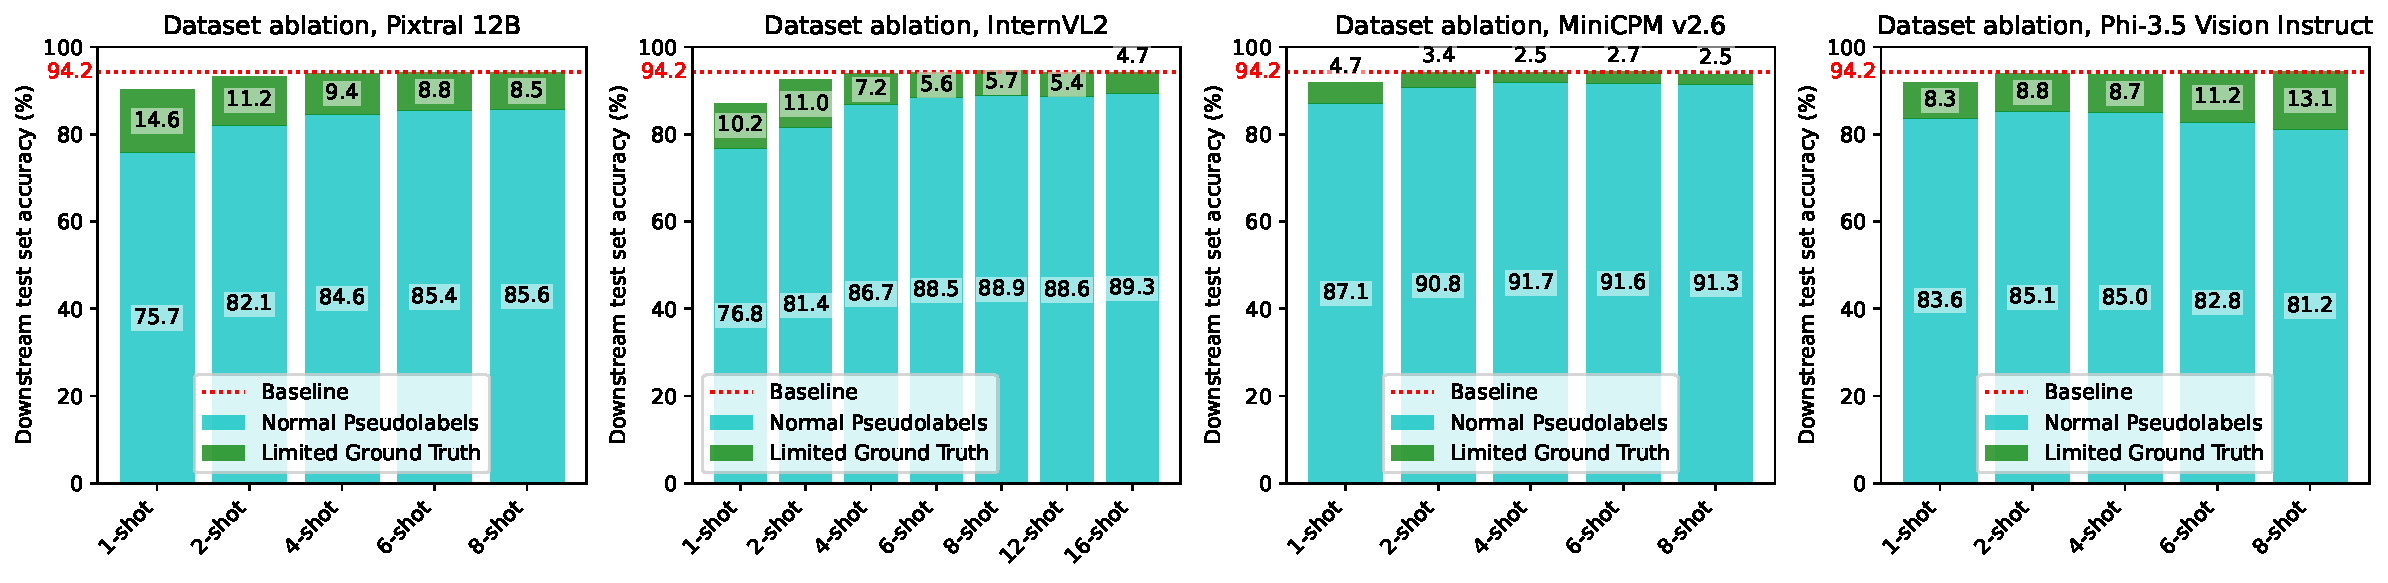
\includegraphics[width=\linewidth]{figures/cifar_downstream_model_accuracy_delta_limited_gt_over_normal.pdf}
    \caption{Visualization of drop in performance of the downstream model caused by noise in pseudolabels generated by the \glspl{vlm}. Limited ground truth data uses the ground truth labels from the dataset for examples that were not invalid in the pseudolabeled dataset.}
    \label{fig:cifar_downstream_model_accuracy_delta_limited_gt_over_normal}
\end{figure*}

\subsubsection{Limitations and Practical Implications}
Context length limitations emerged as a primary constraint, restricting the feasibility of high-shot experiments for several models. Additionally, memory constraints also proved to be a limiting factor, making it impractical to conduct experiments beyond 8 shots for most models. Performance degradation was observed when models were presented with longer inputs or increased numbers of examples, suggesting scalability challenges. A particularly notable issue was the generation of invalid labels, which was especially prevalent in pure few-shot scenarios, impacting the quantity, quality and usability of the generated pseudolabels.

The findings from this study yield several practical implications for implementing \glspl{vlm} in real-world applications. The analysis suggests that zero-shot or low-shot approaches (using 1-2 examples) combined with prompting represent the most efficient implementation strategy. This recommendation is supported by the observation that higher shot counts, while requiring significantly more computational resources, offer diminishing returns in terms of performance gains. For the specific case of the CIFAR-10 dataset, simpler prompts without reasoning requirements proved more effective. Perhaps most notably, downstream models demonstrated remarkable resilience to label quality, suggesting their potential utility in practical applications even with imperfect training data.

\subsection{Seven-Point Checklist Dermatology Dataset (Derm7Pt)}
\label{subsec:evaluation:derm7pt}
The Derm7Pt evaluation encompasses a comprehensive analysis of five \glspl{vlm} on the dermatological image classification task: Pixtral 12B, InternVL2, MiniCPM v26, Phi 3.5 Vision Instruct, and the Biomedical Multimodal Model. The experimental framework includes zero-shot, few-shot, and their variants with clinical images, providing a detailed assessment of model capabilities in medical image interpretation. An overview of the experiment types is provided in \autoref{tab:derm7pt_experiment_types}.

The evaluation methodology for the Derm7Pt dataset incorporates several key adaptations from the CIFAR-10 analysis to accommodate the unique characteristics of medical image classification. First, the dataset utilizes tags to handle the multi-class multiple-classification nature of the dermatological diagnoses. Furthermore, the evaluation framework includes a random accuracy baseline to provide a more meaningful baseline for performance by expressing the accuracy that one might expect to have when making a uniform random guess for the classification of each example in the class-imbalanced categories. A detailed formulation of the metrics can be found in Appendix \ref{sec:appendix:metrics:derm7pt}.

\begin{table}[ht]
    \centering
    \begin{tabular}{p{0.2\linewidth}p{0.6\linewidth}}
        \hline
        \textbf{Experiment Type} & \textbf{Description} \\
        \hline
        \multicolumn{2}{l}{\textit{Diagnosis Experiments}} \\
        0-shot & Basic 0-shot prompting with class lists for direct diagnosis \\
        Reasoning & 0-shot prompting with step-by-step reasoning requirements \\
        Few-shot & Basic prompt with 1-8 examples \\
        \hline
        \multicolumn{2}{l}{\textit{Structured Prompting Experiments}} \\
        0-shot & Separate 0-shot prompting for each of the seven checklist categories \\
        0.5-shot & 0-shot structured prompting enhanced with category-specific information \\
        Few-shot & Basic prompt with 1-8 examples for each category \\
        Few-five shot & Few-shot structured prompting enhanced with category-specific information \\
        \hline
    \end{tabular}
    \caption{Overview of Experiment Types for the Derm7Pt Dataset. Note that each experiment also has variants where clinical images are provided alongside the dermoscopic images, and that the results of the zero-shot experiments in this analysis are best-pooled for brevity. The choice of separating the diagnosis and structured prompting experiments is based on the work of Kawahara et al.~\cite{Kawahara2019}.}
    \label{tab:derm7pt_experiment_types}
\end{table}

\subsubsection{Diagnosis Experiments}
In diagnosis experiments, the model is prompted to generate a direct diagnosis given an image and the grouped class list provided by Kawahara et al.~\cite{Kawahara2019} in their dataset library.

\paragraph{0-shot Diagnosis Experiments}
Initial 0-shot diagnosis experiments revealed significant challenges in model performance. Most models performed notably close to random-guessing accuracy, with only Pixtral 12B performing notably better. Notably, the Biomedical Multimodal Model, despite its domain-specific training, achieved particularly poor results with approximately 2\% accuracy in specific 0-shot scenarios. The introduction of reasoning capabilities generally resulted in decreased performance rather than improvement (except in the case of the Biomedical Multimodal Model), and the inclusion of clinical images often led to a reduction in performance. While computational resource requirements remained relatively stable in terms of memory usage, the addition of reasoning requirements in the prompt led to substantial increases in processing time, with the Pixtral 12B for example experiencing an 82-fold increase in computation time. The best-performing result for each model in the 0-shot diagnosis experiments is used as an additional baseline for the few-shot diagnosis experiments along with the random-guessing baseline.

\paragraph{Few-shot Diagnosis Experiments}
The few-shot diagnostic experiments reveal a persistent performance trend in comparison with the 0-shot diagnosis experiments, with some variation between models. Models are generally able to improve over their 0-shot performance, except in the case of Pixtral 12B, which remains close to but lower than its already higher 0-shot performance. While InternVL2 improves significantly over its 0-shot performance, MiniCPM and Phi 3.5 still perform only slightly better than the random-guessing accuracy. As illustrated in \autoref{fig:derm7pt_few_shot_diagnosis_clinical_over_derm}, the inclusion of clinical images not only failed to improve performance but often proved detrimental to model accuracy, particularly in higher-shot scenarios. The Biomedical Multimodal Model, despite its domain-specific training, demonstrated particularly poor performance and encountered significant difficulties in scenarios with higher shot counts along with context length limitations.

\begin{figure*}[ht]
    \centering
    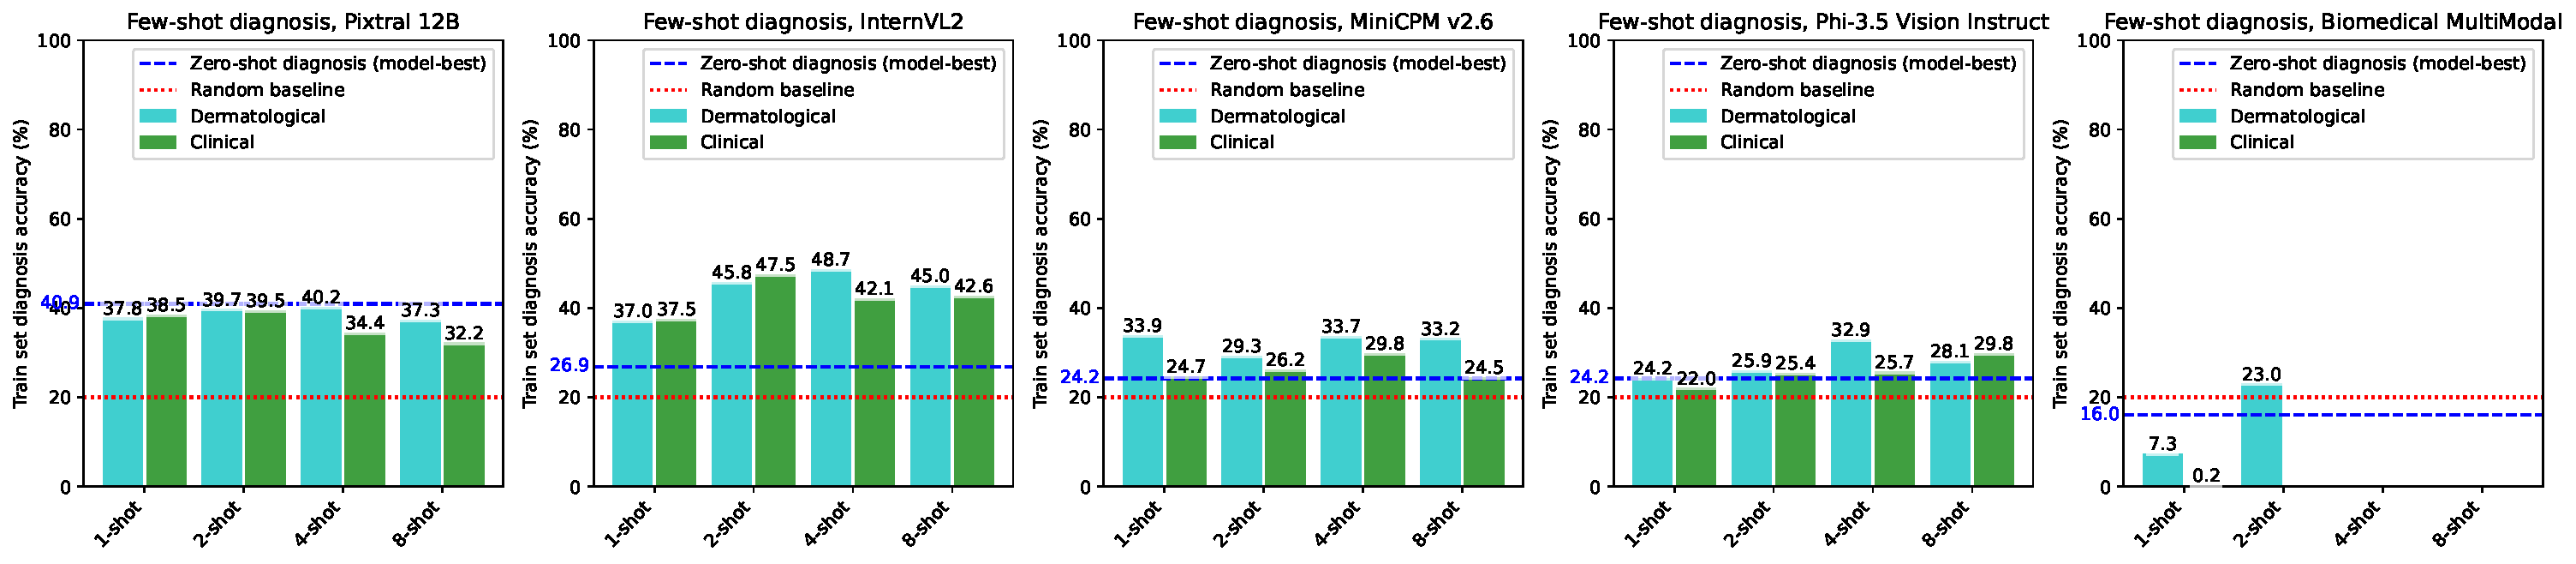
\includegraphics[width=\linewidth]{figures/derm7pt_few_shot_diagnosis_clinical_over_derm.pdf}
    \caption{Visualization of \gls{vlm} performance in few-shot diagnosis experiments. Note the drop in performance of the \gls{vlm} with the additional provision of clinical images over the provision of only dermatological images. The performance of the \gls{vlm} is generally worse when the clinical images are provided, but perform generally on the level of or better than the 0-shot diagnosis performance. The Biomedical Multimodal Model fails outright when provided with clinical images. The Pixtral 12B model has similar performance 0-shot and few-shot, while the other models are generally able to improve over their 0-shot performance.}
    \label{fig:derm7pt_few_shot_diagnosis_clinical_over_derm}
\end{figure*}

\subsubsection{Structured Prompting Experiments}
In structured experiments, the seven categories that make up the Seven-Point Checklist are structured as separate classification problems, and the model is prompted with distinct prompts to make predictions using the grouped class lists from the Seven-Point Checklist Dataset library~\cite{Kawahara2019} for each of the seven multi-class classification problems. The simple average of the accuracies on each of the seven categories is used as the performance metric for the structured experiments.

\paragraph{0-shot Structured Experiments}
The structured 0-shot experiments again revealed persistent challenges across all evaluated models, with models generally performing at or around the random-guessing accuracy. The impact of adding reasoning requirements varied notably across models: Pixtral 12B and InternVL2 showed improved performance when reasoning was incorporated into their prompts, while MiniCPM and Phi 3.5 performed better without reasoning components, as shown in \autoref{fig:derm7pt_zero_five_over_zero_shot_structured}. Particularly noteworthy was the Biomedical Multimodal Model's complete failure in 0-shot scenarios without reasoning, highlighting significant limitations in its base instruction-following capabilities. Even in cases where reasoning was applied, the performance of this model remained below random-guessing accuracy.

\paragraph{0.5-shot Structured Experiments}
The introduction of additional task-specific information in 0.5-shot experiments yielded mixed results. In general, a modest improvement over basic 0-shot performance is observed for most models, with most experiments performing better than random guessing. Notably, Phi 3.5's performance actually deteriorated with the addition of this extra feature information, as shown in \autoref{fig:derm7pt_zero_five_over_zero_shot_structured}. The Biomedical Multimodal Model continues to struggle, maintaining performance levels below random guessing.

\begin{figure*}[ht]
    \centering
    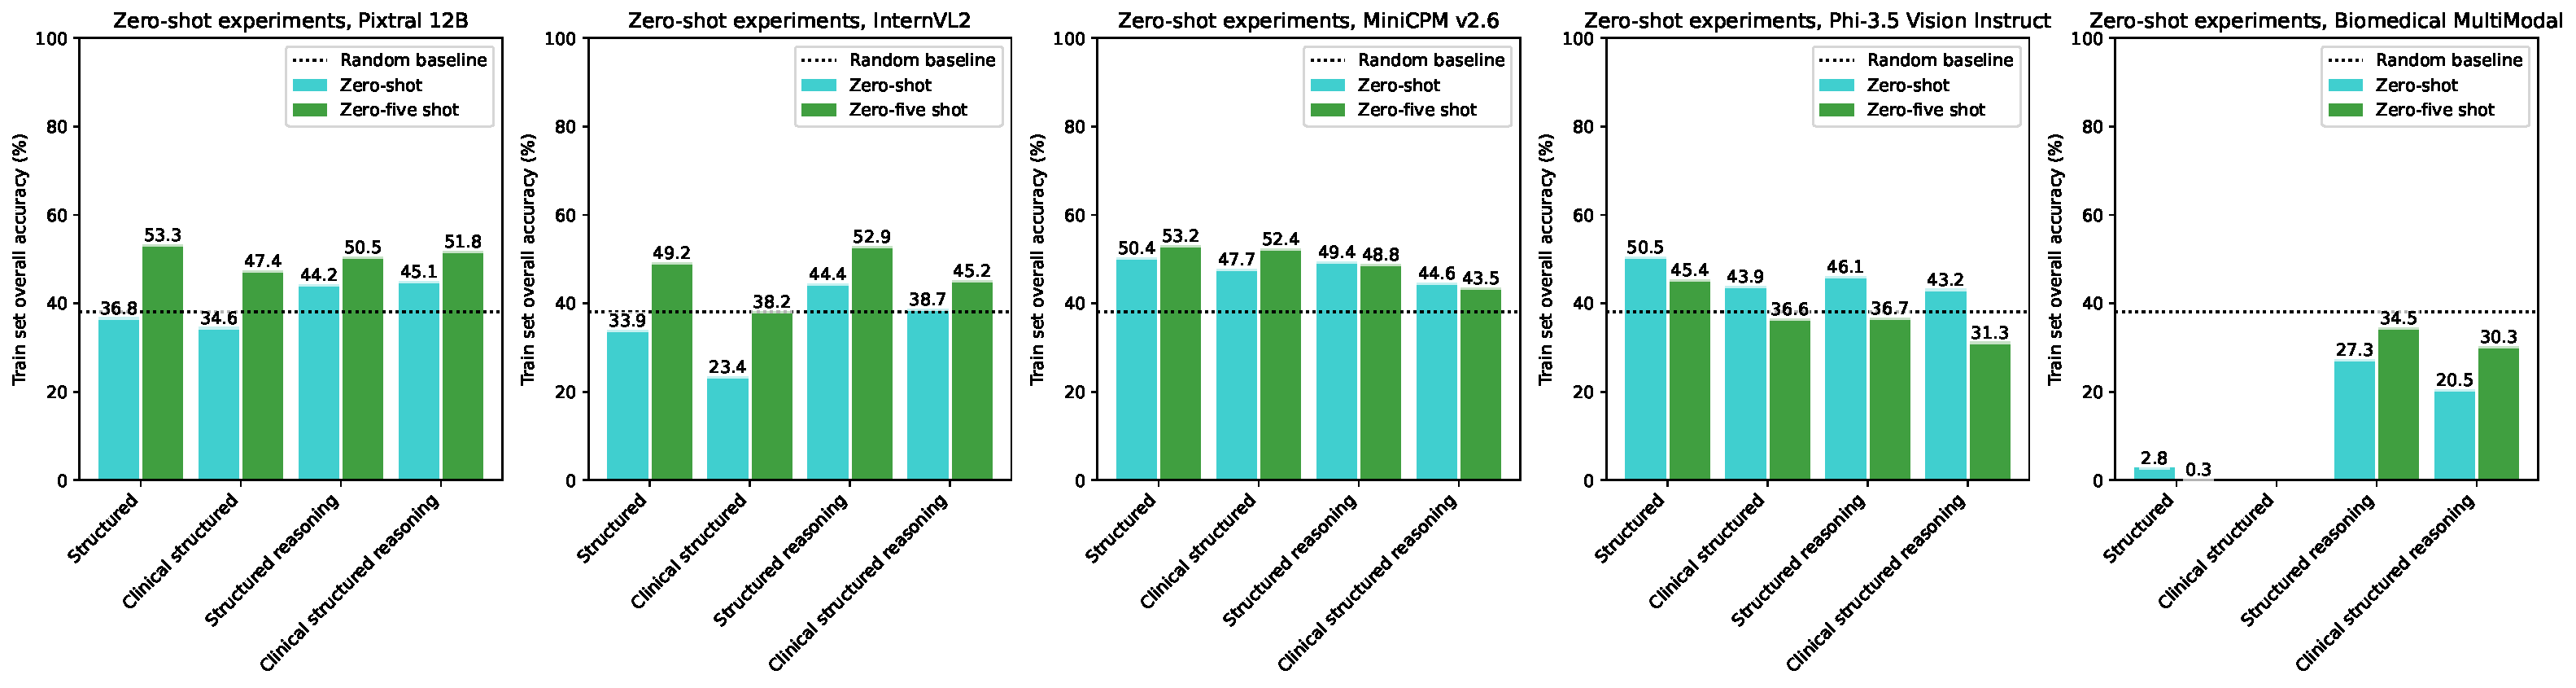
\includegraphics[width=\linewidth]{figures/derm7pt_zero_five_over_zero_shot_structured.pdf}
    \caption{Visualization of the improvement in performance of the \gls{vlm} with the addition of task-specific information in the prompt (0.5-shot) over the base 0-shot performance, using random-guessing performance as a baseline. Note again that the performance of the \glspl{vlm} when provided with clinical images is generally worse than when provided with only dermatological images. In case of the Phi 3.5 model, performance is worse with the additional information in the prompt. Biomedical Multimodal Model fails in scenarios without reasoning as it is unable to output the answer alone.}
    \label{fig:derm7pt_zero_five_over_zero_shot_structured}
\end{figure*}

\paragraph{Few-shot Structured Experiments}
The structured few-shot experiments revealed performance patterns that were generally inferior to the model-best zero-shot structured experiments taken as baselines. Individual models exhibited distinct behavioral patterns: the Biomedical Multimodal Model showed some improvement compared to its zero-shot performance overall (which was significantly worse than random guessing to begin with), while Pixtral 12B demonstrated peak few-shot performance at 2-4 shots before a decline in performance. InternVL2 shows continuous improvement up to 8 shots, whereas other models displayed declining performance as the number of shots increased. These performance patterns, particularly the performance impact when clinical images are also provided are illustrated in \autoref{fig:derm7pt_few_shot_structured_clinical_over_derm}. The performance of the \gls{vlm} is generally worse when clinical images are provided. Memory usage increased with the number of shots in trend similar to that seen in the CIFAR-10 dataset, with this effect being particularly pronounced (increasing by a factor of 1-1.75) when clinical images were included compared to the provision of only dermatological images. This is likely due to the fact that the addition of clinical images in effect doubles the number of images given to the model. The computational demands were also notable, with clinical experiments requiring 1.5-2.5 times longer processing time compared to standard experiments. Since the analysis produces similar results to the CIFAR-10 dataset, the visualizations are not shown here.

\begin{figure*}[ht]
    \centering
    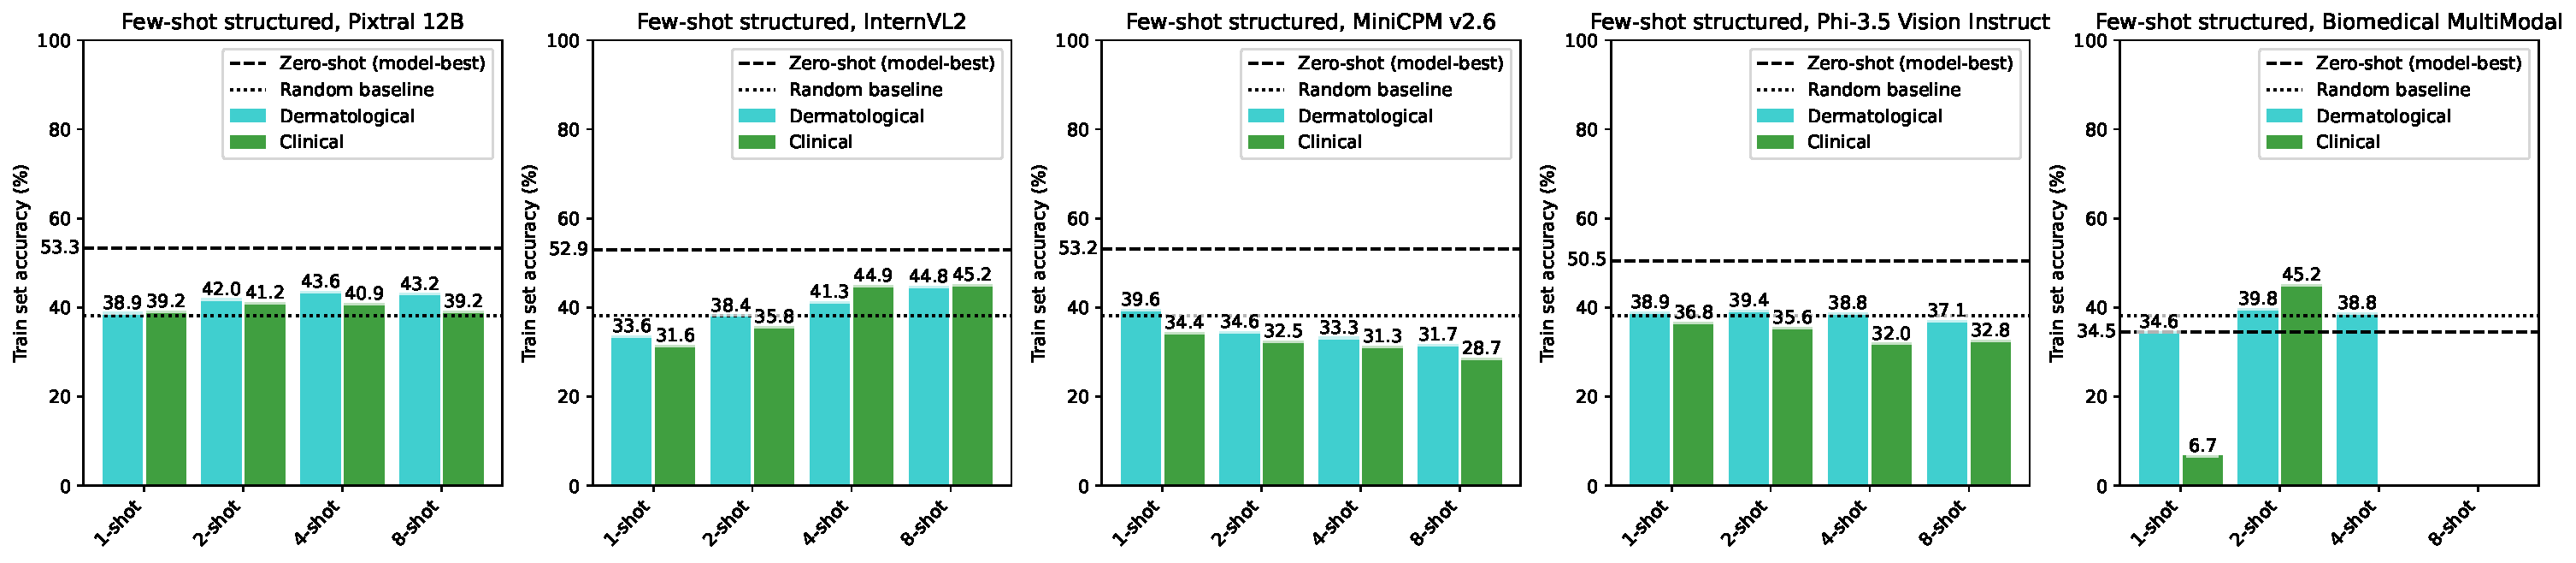
\includegraphics[width=\linewidth]{figures/derm7pt_few_shot_structured_clinical_over_derm.pdf}
    \caption{Visualization of \gls{vlm} performance in few-shot structured experiments in comparison to a zero-shot-best baseline. The drop in performance of the \gls{vlm} with the addition of clinical images over the provision of only dermatological images in structured few-shot experiments is notable. The performance of the \gls{vlm} is generally worse when clinical images are provided.}
    \label{fig:derm7pt_few_shot_structured_clinical_over_derm}
\end{figure*}

\paragraph{Few-five Shot Structured Experiments}
The addition of task-specific information few-shot in few-five shot experiments yielded limited benefits over the few-shot experiments, with overall performance generally remaining at or around random-guessing levels, and below the best zero-shot scenarios. While Pixtral 12B demonstrated slight improvements overall over its corresponding few-shot scenarios and both Pixtral 12B and InternVL2 showed marginal gains in low-shot scenarios, other models exhibited no significant performance changes. Notably, the performance decline with increasing shots observed in few-shot experiments persisted in these few-five shot experiments, as shown in \autoref{fig:derm7pt_few_five_over_few_shot_structured_derm}.

\begin{figure*}[ht]
    \centering
    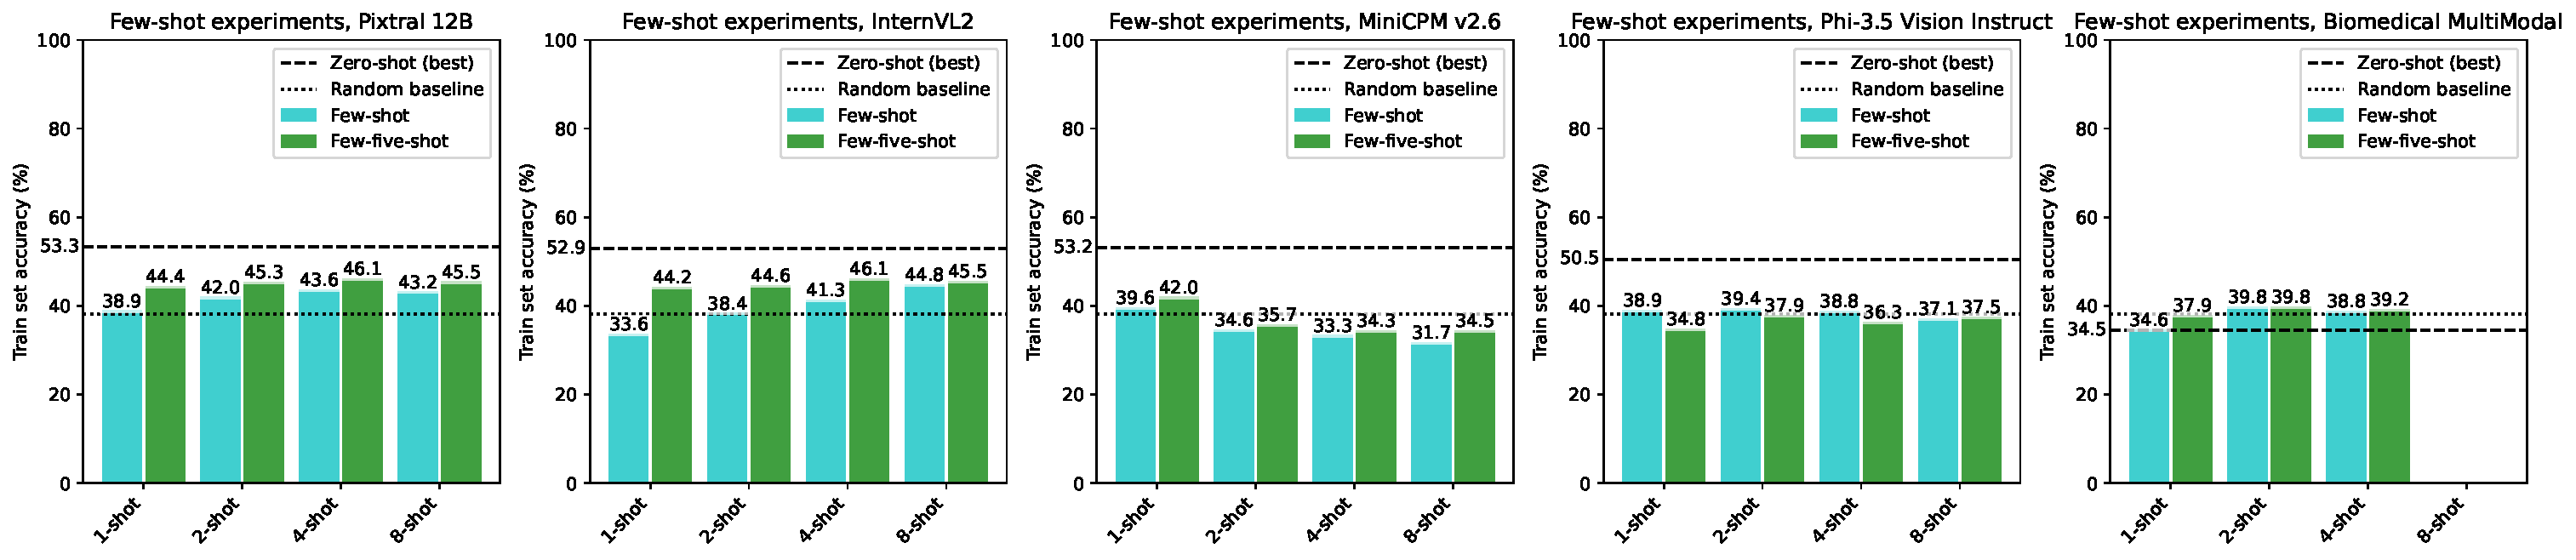
\includegraphics[width=\linewidth]{figures/derm7pt_few_five_over_few_shot_structured_derm.pdf}
    \caption{Visualization of the performance of the \gls{vlm} with the addition of task-specific information in the prompt (few-five shot) over the baseline few-shot performance. Note that the performance of the \glspl{vlm} when provided with clinical images is generally worse and is hence not considered further in this plot.}
    \label{fig:derm7pt_few_five_over_few_shot_structured_derm}
\end{figure*}

\subsubsection{Challenges and Limitations}
The analysis reveals significant challenges in applying \glspl{vlm} to specialized medical imaging tasks:
\begin{enumerate}[label=\alph*)]
    \item Performance across all models are consistently at or around random-guessing accuracy, indicating fundamental limitations in their ability to handle specialized medical classification tasks. Few-shot performance generally improved upon zero-shot performance in diagnosis experiments, while zero-shot performance was better overall in structured prompting experiments.
    
    \item The incorporation of additional clinical images alongside dermatological images not only failed to improve performance but often led to degraded accuracy, suggesting challenges in integrating multiple image modalities.
    
    \item Increasing the complexity of model inputs through additional shots or reasoning requirements typically resulted in decreased performance, contrary to the expected benefits of additional reasoning context for the model in making a classification.
    
    \item Computational resource requirements increased substantially with experiment complexity, with both memory usage and processing time scaling non-linearly as more shots or clinical images were added.
    
    \item Even specialized models like the Biomedical Multimodal Model, despite being specifically fine-tuned for medical tasks, struggled significantly with the classification problem (as seen in \autoref{fig:derm7pt_model_best_performance_over_model_parameter_count}).
\end{enumerate}

\begin{figure}[ht]
    \centering
    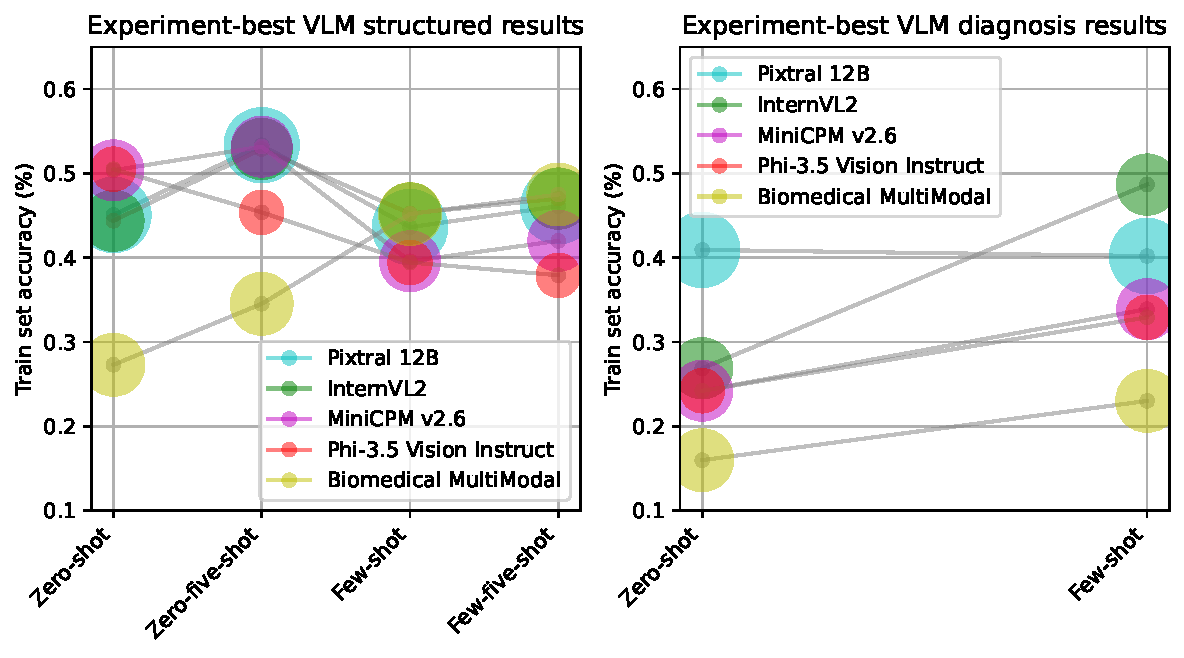
\includegraphics[width=\linewidth]{figures/derm7pt_model_best_performance_over_model_parameter_count.pdf}
    \caption{Visualization of the best performance of each model scaled by the number of parameters in the model. Note that the performance of the models does not necessarily correlate with the number of parameters in the model, and a domain-specific fine-tuned model generally performed poorly in this analysis.}
    \label{fig:derm7pt_model_best_performance_over_model_parameter_count}
\end{figure}

This suggests that current \glspl{vlm} may not be feasible for specialized medical imaging tasks without significant improvements or specialized training. This reiterates on the observation that few-shot in-context learning requires language models to have some knowledge of the task from pre-training~\cite{Brown2020}, and as such, does not perform well with the models investigated here.

\subsection{Summary of Findings}
The comprehensive evaluation of \glspl{vlm} across both CIFAR-10 and specialized medical imaging tasks revealed several key insights about their few-shot learning capabilities and practical applications:

Model performance was seen to show strong task dependence. For image classification on CIFAR-10, a task likely covered in pre-training, models demonstrated reasonable performance with downstream models even outperforming the \glspl{vlm} themselves. However, on the specialized Derm7Pt dataset, performance was consistently at random-guessing levels, highlighting the crucial role of pre-existing task knowledge for the success of few-shot in-context learning.

The relationship between input complexity and performance was notably consistent across both tasks. Adding more shots or reasoning requirements often led to decreased performance rather than improvements, while significantly increasing computational costs. This suggests that simpler prompting strategies (zero-shot or low-shot with 1-2 examples along with a prompt) may be more practical for real-world applications.

Model architecture and training background appear to significantly influence performance patterns. Models trained on multi-turn, multi-image conversations show different performance scaling behaviors with the provision of examples in input compared to models focused on single-image tasks like visual question answering, image captioning, and conversational tasks. However, larger model size did not necessarily correlate with better performance, as evidenced by the varying performance across model scales and the observed poor performance of domain-specific models on specialized tasks.

These experiments revealed important practical considerations for deploying these models. While downstream models showed remarkable resilience to label quality in CIFAR-10 experiments, the challenges in specialized task domains suggest that current \glspl{vlm} require significant improvements or specialized training before they can be reliably applied to domain-specific tasks like the medical imaging task investigated here.

\end{document}
